% Welcome! This is the unofficial University of Udine beamer template.

% See README.md for more informations about this template.

% This style has been developed following the "Manuale di Stile"
% (Style Manual) of the University of Udine. You can find the
% manual here: https://www.uniud.it/it/ateneo-uniud/ateneo-uniud/identita-visiva/manuali-immagine-stile/manuale-stile

% Note: for some reason, the RGB values specified in the manual
% do NOT render correctly in Beamer, so they have been redefined
% for this document using the high level chromo-optic deep neural 
% quantistic technology offered by Microsoft Paint's color picker.

% We defined four theme colors: UniBrown, UniBlue, UniGold
% and UniOrange. For example, to write some uniud-brownish
% text, just use: \textcolor{UniBrown}{Hello!}

% Note that [usenames,dvipsnames] is MANDATORY due to compatibility
% issues between tikz and xcolor packages.

\documentclass[usenames,dvipsnames,aspectratio=169]{beamer}
\usepackage[utf8]{inputenc}
\usepackage{verbatim}
\usetheme{uniud}

%%% Bibliography
\usepackage[style=authoryear,backend=biber]{biblatex}
\addbibresource{bibliography.bib}

% Author names in publication list are consistent 
% i.e. name1 surname1, name2 surname2
% See https://tex.stackexchange.com/questions/106914/biblatex-does-not-reverse-the-first-and-last-names-of-the-second-author
\DeclareNameAlias{author}{first-last}

%%% Suppress biblatex annoying warning
\usepackage{silence}
\WarningFilter{biblatex}{Patching footnotes failed}

%%% Some useful commands
% pdf-friendly newline in links
\newcommand{\pdfnewline}{\texorpdfstring{\newline}{ }} 
% Fill the vertical space in a slide (to put text at the bottom)
\newcommand{\framefill}{\vskip0pt plus 1filll}


\title[Introduction to Gaussian Processes]{Introduction to \\ Gaussian Processes}
\date[May 1977]{\today}
\author[Filipe P. de Farias]{
  Filipe P. de Farias, IC
  \pdfnewline
  \texttt{filipepfarias@fisica.ufc.br}
}
\institute{Teleinformatics Engineering Department, Federal University of Ceará}

\begin{document}
\begin{frame}
\titlepage
\end{frame}

\begin{frame}{Preamble} 
 The \textcolor{white}{\marker[UniBrown]{ Gaussian Processes }} are the widely used stochastic processes for modeling dependent data observed over time, space or even time and space. Here, we'll iniciate our study with a \textbf{Probability and Random Process Theory Review} taking some points to base our journey, going through \textbf{Linear Regression} and finally the GP.
\end{frame}

\begin{frame}{Outline}
\tableofcontents
\end{frame}

\section{Probability and Random Process Theory Review}
\subsection{Basic Concepts of Probability Theory}
\framecard{\insertsection}


\begin{frame}{\insertsubsection}

\end{frame}



\begin{frame}{Overleaf users}

\begin{alertblock}{Warning}
You can ignore this slide if you're \textbf{not} working with Overleaf.
\end{alertblock}

\vskip 0.5cm

Overleaf, Beamer and Biber do not always get along well together. For this reason, if you make a mistake while writing this presentation, in the drop-down error message you'll \textbf{always} get Biber-related error messages.

\vskip 0.5cm

Luckily, you just have to click on ``\texttt{go to first error/warning}'' and the UI will scroll to the line containing your mistake.

\end{frame}

\begin{frame}[fragile]
\frametitle{Compiling}

\begin{alertblock}{Warning}
You can ignore this slide if you're working with Overleaf.
\end{alertblock}

To compile this deck you'll need the \texttt{biber} package. Probably your \TeX editor already supports it; if not, you will easily find online the instructions to install it.

\vskip 0.5cm

If you're not using an editor, you can compile this presentation using the command line by running:

\begin{verbatim}
$ pdflatex main.tex
$ biber main.bcf
$ pdflatex main.tex
$ pdflatex main.tex
\end{verbatim}


\end{frame}


%\section{Introduction to Curve Fitting}
%\section{Linear Regression}
\framecard{\insertsection}
\subsection{Basic Concepts of Curve Fitting}

%
%

\subsection{Bayesian Curve Fitting}
\begin{frame}{\insertsubsection}
	\visible<1->{So, we'll start to look the regression with a statistical approach. To encourage you, let's take the sentence.}
	\visible<2>{\vspace{1.5em}
		\begin{block}{Sentence}
		\textit{If we could update the \textbf{\textcolor{red}{regression weights}} as we acquire some new values of the experiment?}
		\end{block}
   		     }
\end{frame}

\begin{frame}{\insertsubsection}
	\visible<1->{Let's take a look again at the Bayes Theorem}
	
	\visible<2->{
	\begin{block}{Bayes Theorem}{
			\begin{equation}\label{bayes_theorem}
				\visible<2->{ p(\mathbf{w}|\mathcal{D}) = \frac{p(\mathcal{D}| \mathbf{w}) \overbrace{ p(\mathbf{w})}^{\mathclap{\text{the \textit{a priori} probability}}}} { \underbrace{ p(\mathcal{D})}_{\mathclap{\text{the \textit{a priori} probability}}}} } 
			\end{equation}
			}
	\end{block}
	\visible<3->{So, if\textbf{ we have the probability} of the data, we'll could estimate the\textbf{ future weights}.}
	\visible<4>{\centering\textbf{\textcolor{red}{But, how?}}}
	}
\end{frame}

\begin{frame}{\insertsubsection}
	\visible<1->{Taking some steps back, let's re-visit the \textbf{Curve Fitting}. There, the strategy was minimize the error function.\vspace{1.5em} \\}
	\visible<2->{Now we'll try to view the same problem with a \textit{probabilistic perspective}. We're trying to make predictions for the target value $\boldsymbol{t}$ given some new values of $x$.\vspace{1.5em} \\}
	\visible<3->{A good ideia is to express our target values $\boldsymbol{t}$ in terms of \textbf{gaussians distributions} with the mean equals to $y(x,\mathbf{w})$.}
\end{frame}

\begin{frame}{\insertsubsection}
	\begin{figure}
		\label{schematic-gaussian-distribution}
		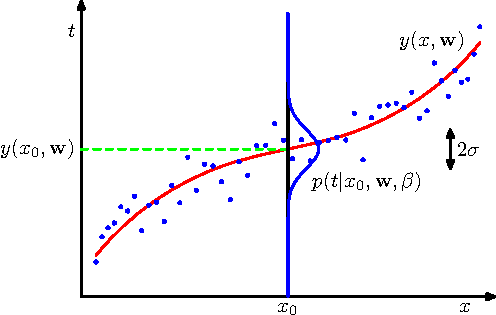
\includegraphics[totalheight=0.6\textheight]{Figure1c16.pdf}
		\caption{Schematic of the polynomial function $y(x,\mathbf{w})$ and the gaussian distribution $p$.}

	\end{figure}
\end{frame}


\begin{frame}{Title}
  $
    blah =
    \only<1>{blah}
    \only<2>{result}
    \visible<1>{%
      =
      \begin{cases}
          blah \\ 
          blah
        \end{cases}
      }
    $
\end{frame}

\end{document}